\chapter{प्रोटॉन NMR}\label{ch:g12:proton-nmr}

किसी अस्पताल में एक रोगी MRI स्कैनर के छल्ले के भीतर लेटा है, और स्क्रीन पर
शरीर के कोमल ऊतकों का एक चित्र प्रकट होता है, जो उसके पानी और वसाओं के
हाइड्रोजन \omterm{def:g9:inside-the-atom:nucleus}{नाभिकों} के उत्तरों से बना है। रसायन की किसी
प्रयोगशाला में, किसी यौगिक के कुछ मिलीग्राम वाली काँच की एक छोटी नली
एक शक्तिशाली चुंबक के छिद्र में उतारी जाती है, और उसी तरह बना एक स्पेक्ट्रम
प्रकट होता है: एक प्रबल चुंबक, एक रेडियो संकेत, और उसका उत्तर देते
हाइड्रोजन \omterm{def:g9:inside-the-atom:nucleus}{नाभिक}। रसायनज्ञ के स्पेक्ट्रममापी में हर हाइड्रोजन \omterm{def:g9:inside-the-atom:nucleus}{नाभिक} अपने
पड़ोसियों के अनुसार थोड़ा अलग उत्तर देता है, और स्पेक्ट्रम \omterm{def:g7:atoms-and-molecules:molecule}{अणु} के
हाइड्रोजन \omterm{def:g7:atoms-and-molecules:atom}{परमाणुओं} का एक मानचित्र होता है।

\begin{recall}
\omterm{def:g11:infrared:spectrum}{अवरक्त स्पेक्ट्रम} दिखाता है कि किसी \omterm{def:g7:atoms-and-molecules:molecule}{अणु} में कौन-से आबंध हैं
(\cref{ch:g11:infrared})। \omterm{def:g11:functional-groups:functional-group}{क्रियात्मक समूह}, परिवार और \omterm{def:g11:organic-skeletons:isomer}{समावयवी}
(\cref{ch:g11:functional-groups}, \cref{ch:g11:organic-skeletons})।
\end{recall}

\begin{omfigure}
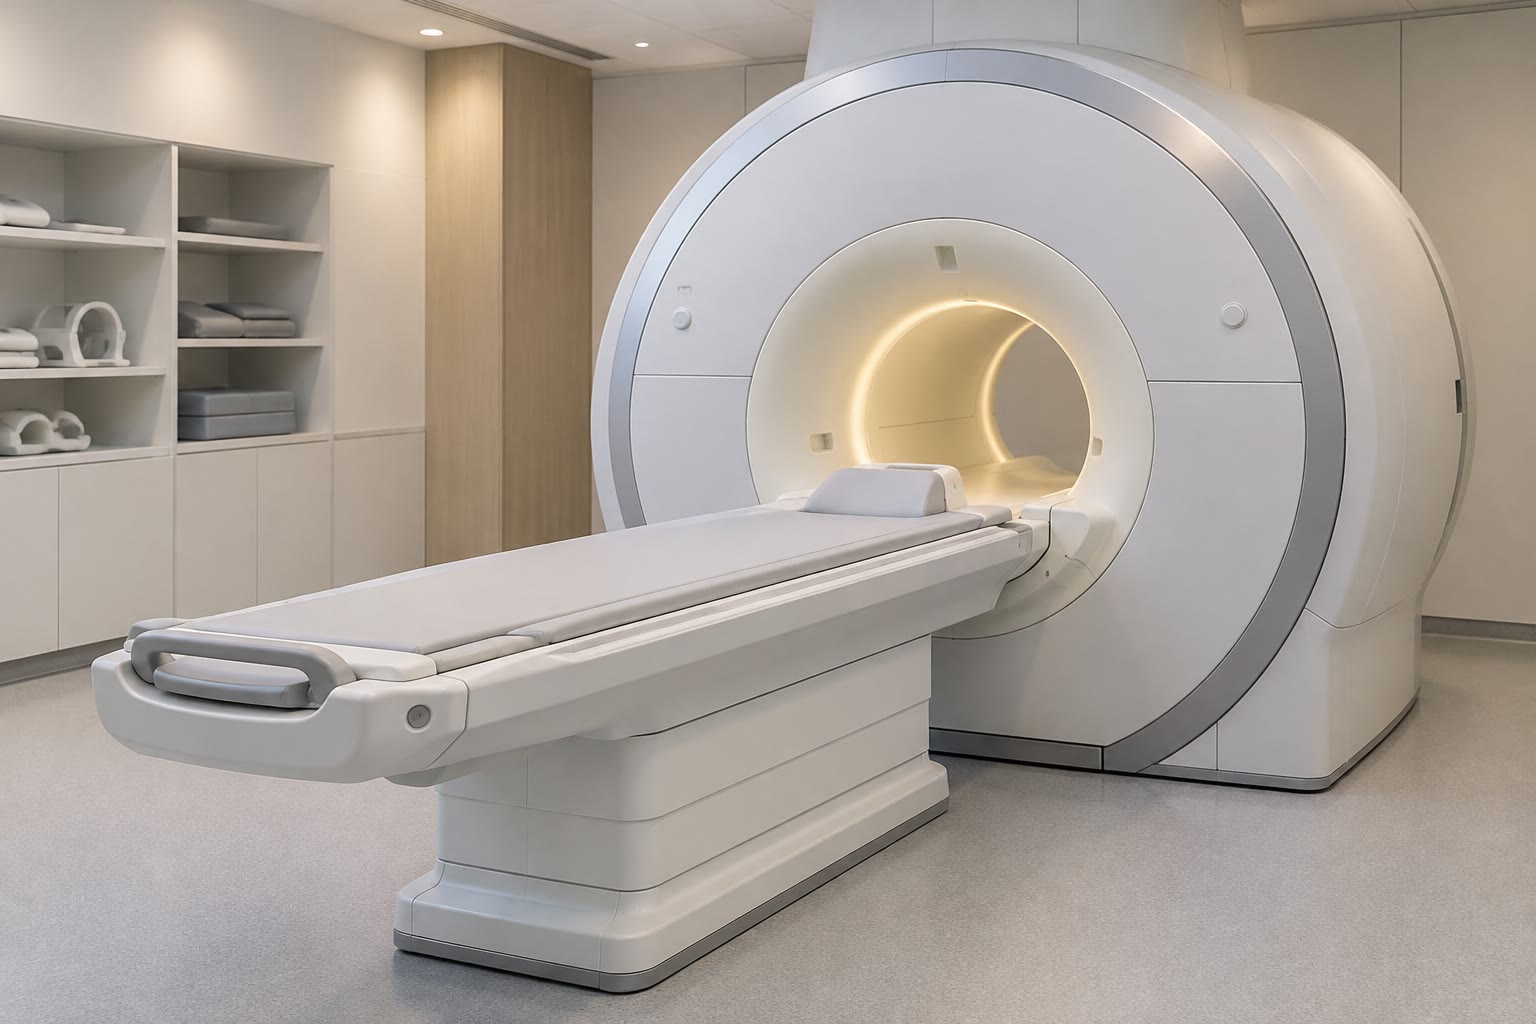
\includegraphics[width=0.48\linewidth]{images/book1/ai/g12-mri-room.jpg}

{\small एक MRI स्कैनर: वही भौतिकी जो रसायनज्ञ के NMR
स्पेक्ट्रममापी की है।}
\end{omfigure}

\section{चुंबकीय क्षेत्र में प्रोटॉन}

हाइड्रोजन \omterm{def:g7:atoms-and-molecules:atom}{परमाणु} का \omterm{def:g9:inside-the-atom:nucleus}{नाभिक} एक अकेला \omterm{def:g9:inside-the-atom:proton}{प्रोटॉन} है। प्रबल
चुंबकीय क्षेत्र में रखे जाने पर वह एक सटीक आवृत्ति की रेडियो तरंगें अवशोषित करता है; कैसे और
क्यों, यह भौतिकी का विषय है, और यहाँ आवश्यक नहीं। रसायनज्ञ के लिए
महत्त्वपूर्ण यह है कि \omterm{def:g9:inside-the-atom:proton}{प्रोटॉन} के चारों ओर के \omterm{def:g9:inside-the-atom:nucleus}{इलेक्ट्रॉन} उसे क्षेत्र से थोड़ा
परिरक्षित करते हैं, और यह परिरक्षण पास के \omterm{def:g7:atoms-and-molecules:atom}{परमाणुओं} पर निर्भर करता है: \omterm{def:g9:inside-the-atom:nucleus}{इलेक्ट्रॉनों} को
दूर खींचने वाले किसी विद्युत-ऋणात्मक ऑक्सीजन \omterm{def:g7:atoms-and-molecules:atom}{परमाणु} के बगल का \omterm{def:g9:inside-the-atom:proton}{प्रोटॉन}
हाइड्रोकार्बन श्रृंखला के \omterm{def:g9:inside-the-atom:proton}{प्रोटॉन} से थोड़ी अलग आवृत्ति पर अवशोषित करता है।
ये अंतर बहुत छोटे होते हैं, आवृत्ति के कुछ दस-लाखवें भाग, और इन्हें
प्रति दस लाख भाग में दिया जाता है।

\begin{omfigure}
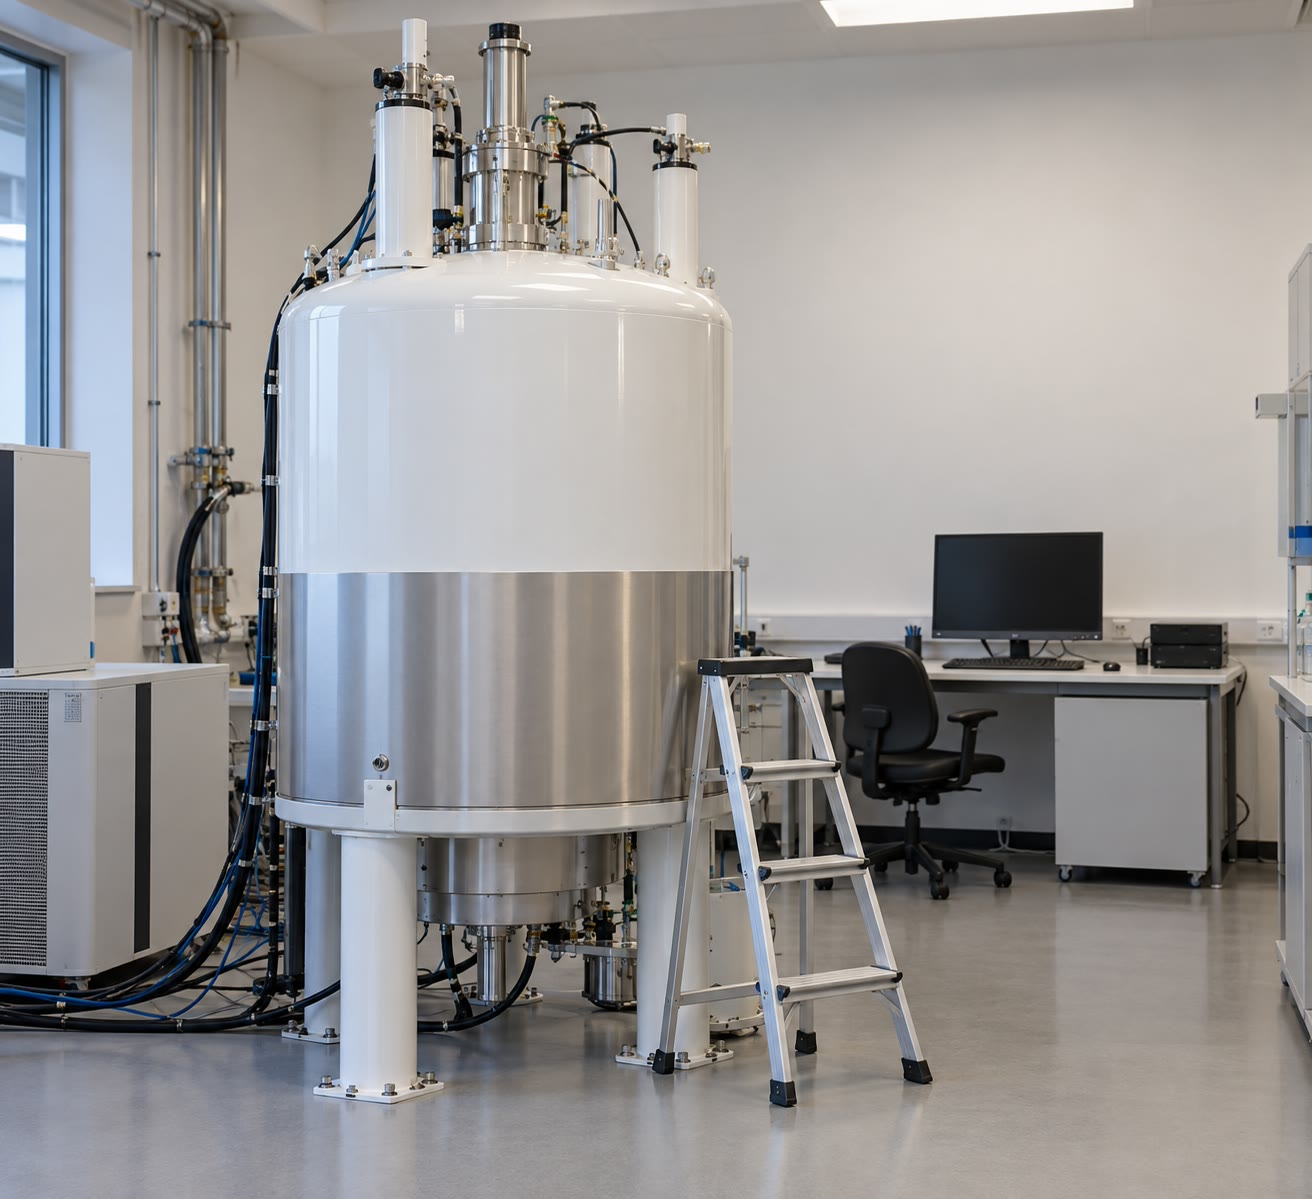
\includegraphics[width=0.42\linewidth]{images/book1/ai/g12-nmr-magnet.jpg}

{\small एक NMR स्पेक्ट्रममापी का चुंबक।}
\end{omfigure}

\begin{definition}[NMR स्पेक्ट्रम, रासायनिक विस्थापन]\label{def:g12:proton-nmr:spectrum}
\omterm{def:g9:inside-the-atom:proton}{प्रोटॉन} \emph{NMR स्पेक्ट्रम}\index{NMR स्पेक्ट्रम} (नाभिकीय चुंबकीय
अनुनाद) किसी यौगिक के हाइड्रोजन \omterm{def:g9:inside-the-atom:nucleus}{नाभिकों} द्वारा अवशोषित संकेत दिखाता है।
किसी संकेत की स्थिति उसका \emph{रासायनिक
विस्थापन}\index{रासायनिक विस्थापन} $\delta$ है, प्रति दस लाख भाग (\si{ppm}) में,
जिसे एक संदर्भ यौगिक, टेट्रामेथिलसिलेन
\ce{Si(CH3)4} (TMS), के संकेत से मापा जाता है, जो $\delta = 0$ पर रखा जाता है। $\delta$ अक्ष
दाएँ से बाएँ बढ़ता हुआ बनाया जाता है।
\end{definition}

\begin{proposition}[विस्थापन पड़ोसियों पर निर्भर करता है]\label{prop:g12:proton-nmr:shift}
% ledger: nmrr:CH3, nmrr:CH2, nmrr:allylic, nmrr:ketone, nmrr:halide, nmrr:alcohol, nmrr:vinylic, nmrr:aryl, nmrr:aldehyde, nmrr:acid
किसी \omterm{def:g9:inside-the-atom:proton}{प्रोटॉन} का \omterm{def:g12:proton-nmr:spectrum}{रासायनिक विस्थापन} उसके पास के \omterm{def:g7:atoms-and-molecules:atom}{परमाणुओं} पर निर्भर करता है: वह
किसी विद्युत-ऋणात्मक \omterm{def:g7:atoms-and-molecules:atom}{परमाणु} या \omterm{def:g10:lewis-and-shape:multiple-bond}{द्विआबंध} के जितना निकट हो, उसका
विस्थापन उतना ही बड़ा। सामान्य परास, \si{ppm} में:
\begin{center}
\small
\begin{tabular}{ll@{\qquad}ll}
\hline
परिवेश & $\delta$ & परिवेश & $\delta$ \\
\hline
श्रृंखला में \ce{CH3} & 0.7--1.3 & \ce{H-C-O} (\omterm{def:g11:functional-groups:alcohol}{ऐल्कोहॉल}, ईथर, \omterm{def:g11:functional-groups:carboxylic-acid}{एस्टर}) & 3.3--4.5 \\
श्रृंखला में \ce{CH2} & 1.2--1.6 & \ce{H-C=C} & 4.5--6.5 \\
\ce{H-C-C=C} & 1.6--2.2 & बेंज़ीन वलय पर H & 6.5--8.0 \\
\ce{H-C-C=O} & 2.0--2.4 & \omterm{def:g11:functional-groups:carbonyl}{ऐल्डिहाइड} \ce{-CHO} & 9.7--10.0 \\
\ce{H-C-X} (\omterm{def:g10:electron-shells:family}{हैलोजन}) & 2.5--4.0 & अम्ल \ce{-COOH} & 11.0--12.0 \\
\hline
\end{tabular}
\end{center}
\end{proposition}

\begin{proof}
अनेक यौगिकों पर मापा गया। विद्युत-ऋणात्मक पड़ोसी \omterm{def:g9:inside-the-atom:proton}{प्रोटॉन} से
\omterm{def:g9:inside-the-atom:nucleus}{इलेक्ट्रॉनों} को दूर खींचता है, जो कम परिरक्षित होकर
अधिक विस्थापन पर अवशोषित करता है।
\end{proof}

\begin{omfigure}
\begin{tikzpicture}[font=\small, x=0.75cm, y=0.5cm]
  % delta axis reversed: x = 12 - delta
  \draw[->] (0,0) -- (12.4,0) node[right] {};
  \foreach \d in {12,11,10,9,8,7,6,5,4,3,2,1,0}
    \draw ({12-\d},0) -- ({12-\d},-0.2) node[below, font=\footnotesize] {\d};
  \node[below=14pt] at (6,-0.3) {$\delta$ (\si{ppm})};
  \foreach \a/\b/\y/\c/\l in {
      11.0/12.0/1/omThm/{\ce{COOH}},
      9.7/10.0/2/omThm/{\ce{CHO}},
      6.5/8.0/1/black!60/{बेंज़ीन वलय},
      4.5/6.5/2/omMeth/{\ce{C=C-H}},
      3.3/4.5/3/omDef/{\ce{H-C-O}},
      2.0/2.4/4/omProp/{\ce{H-C-C=O}},
      0.7/1.6/5/black!45/{श्रृंखलाओं के \ce{CH3}, \ce{CH2}}} {
    \fill[\c, rounded corners=1pt] ({12-\b},{\y-0.3}) rectangle ({12-\a},{\y+0.3});
    \node[anchor=west, font=\footnotesize] at ({12-\a+0.1},\y) {\l};
  }
  \draw[thick] (12,0) -- (12,0.6) node[above, font=\footnotesize] {TMS};
\end{tikzpicture}

{\small परिवेश के अनुसार \omterm{def:g9:inside-the-atom:proton}{प्रोटॉन} कहाँ अवशोषित करते हैं। ऑक्सीजन, \omterm{def:g10:lewis-and-shape:multiple-bond}{द्विआबंध}
या अम्ल समूह के निकट के \omterm{def:g9:inside-the-atom:proton}{प्रोटॉन} स्पेक्ट्रम के बाईं ओर दिखते हैं।}
\end{omfigure}

\begin{inthelab}[NMR नली तैयार करना]
यौगिक के कुछ मिलीग्राम लगभग
\qty{0.6}{mL} ऐसे \omterm{def:g6:solutions-and-solubility:solute}{विलायक} में घोले जाते हैं जिसके हाइड्रोजन \omterm{def:g7:atoms-and-molecules:atom}{परमाणुओं} को
ड्यूटीरियम से बदल दिया गया है (\ce{CDCl3}, ड्यूटेरीकृत क्लोरोफ़ॉर्म), जो कोई संकेत नहीं देता;
संदर्भ के रूप में TMS की सूक्ष्म मात्रा मिलाई जाती है। विलयन को छानकर
काँच की एक पतली नली में भरा जाता है, जिसे ढक्कन लगाकर, लेबल करके चुंबक में उतारा जाता है।
\end{inthelab}

\section{तुल्य प्रोटॉन}

\begin{definition}[तुल्य प्रोटॉन]\label{def:g12:proton-nmr:equivalent}
\omterm{def:g9:inside-the-atom:proton}{प्रोटॉन} \emph{तुल्य प्रोटॉन}\index{तुल्य प्रोटॉन} होते हैं यदि \omterm{def:g7:atoms-and-molecules:molecule}{अणु} में
उनका परिवेश एक-सा हो, ताकि वे एक ही
विस्थापन पर अवशोषित करें। तुल्य \omterm{def:g9:inside-the-atom:proton}{प्रोटॉनों} का हर समूह एक संकेत देता है। किसी
\ce{CH3} समूह के तीनों \omterm{def:g9:inside-the-atom:proton}{प्रोटॉन} सदा तुल्य होते हैं।
\end{definition}

\begin{example}[समूह गिनना]\label{ex:g12:proton-nmr:groups}
प्रोपेनोन, \ce{CH3-CO-CH3}, में छह \omterm{def:g9:inside-the-atom:proton}{प्रोटॉन} हैं पर एक ही समूह: दोनों
\ce{CH3} एक जैसे हैं, \ce{C=O} के दोनों ओर एक-एक। एथेनॉल,
\ce{CH3-CH2-OH}, में तीन समूह हैं (\ce{CH3}, \ce{CH2}, \ce{OH}), और
एथिल एथेनोएट, \ce{CH3-CO-O-CH2-CH3}, में भी तीन: \ce{CH3}, जो
\ce{C=O} के बगल में है; \ce{CH2}, जो \ce{O} के बगल में है; और सिरे पर
\ce{CH3}।
\end{example}

\section{समाकलन}

\begin{definition}[समाकलन वक्र]\label{def:g12:proton-nmr:integration}
किसी \omterm{def:g12:proton-nmr:spectrum}{NMR स्पेक्ट्रम} का \emph{समाकलन वक्र}\index{समाकलन वक्र}
संकेतों के ऊपर बनाया गया एक वक्र है, जो हर संकेत पर एक सीढ़ी जितना ऊपर उठता है:
हर सीढ़ी की ऊँचाई उस संकेत को देने वाले \omterm{def:g9:inside-the-atom:proton}{प्रोटॉनों} की संख्या के
समानुपाती होती है।
\end{definition}

\begin{example}[सीढ़ियाँ पढ़ना]\label{ex:g12:proton-nmr:steps}
एथेनॉल के स्पेक्ट्रम में तीनों संकेतों के ऊपर की सीढ़ियाँ, बाएँ से दाएँ, 2,
1 और 3 इकाई मापती हैं: \ce{CH2}, \ce{OH} और \ce{CH3}। केवल
अनुपात मायने रखते हैं: 12, 6 और 18 mm की सीढ़ियाँ भी यही बात कहती हैं।
\end{example}

\section{बहुकता और \texorpdfstring{$n+1$}{n+1} नियम}


\begin{definition}[बहुक, $n+1$ नियम]\label{def:g12:proton-nmr:multiplet}
कोई संकेत अक्सर कई पास-पास की रेखाओं में विभक्त होता है: एक \emph{बहुक}\index{बहुक}
(एकक, द्विक, त्रिक, चतुष्क, \dots{} 1, 2, 3, 4 रेखाओं के लिए)।
\emph{$n+1$ नियम}\index{n+1 नियम@$n+1$ नियम} के अनुसार, \omterm{def:g12:proton-nmr:equivalent}{तुल्य प्रोटॉनों} का वह समूह
जिसके पड़ोसी कार्बन \omterm{def:g7:atoms-and-molecules:atom}{परमाणुओं} पर कुल $n$ ऐसे \omterm{def:g9:inside-the-atom:proton}{प्रोटॉन} हों जो उसके
तुल्य नहीं, $n+1$ रेखाओं का संकेत देता है, जिनकी तीव्रताएँ
पास्कल त्रिभुज के अनुपातों में होती हैं।
\end{definition}

\begin{proposition}[पड़ोसियों द्वारा विभाजन]\label{prop:g12:proton-nmr:n-plus-one}
\omterm{def:g7:atoms-and-molecules:molecule}{अणु} \ce{CH3-CH2-X} (X हाइड्रोजन रहित) में \ce{CH3} संकेत
एक त्रिक है (2 पड़ोसी \omterm{def:g9:inside-the-atom:proton}{प्रोटॉन}) और \ce{CH2} संकेत एक चतुष्क
(3 पड़ोसी \omterm{def:g9:inside-the-atom:proton}{प्रोटॉन})। ऑक्सीजन या नाइट्रोजन \omterm{def:g7:atoms-and-molecules:atom}{परमाणु} से आबंधित \omterm{def:g9:inside-the-atom:proton}{प्रोटॉन}
आम तौर पर एकक देते हैं और अपने पड़ोसियों को विभक्त नहीं करते।
\end{proposition}

\begin{proof}
स्वीकृत: हर पड़ोसी \omterm{def:g9:inside-the-atom:proton}{प्रोटॉन} अपनी अवस्था के अनुसार संकेत को थोड़ा ऊपर या नीचे
खिसकाता है, और इनके संयोजन $n+1$ रेखाएँ देते हैं; इसकी
भौतिकी विश्वविद्यालय के प्रथम वर्ष के खंड में समझाई गई है। O या N पर स्थित \omterm{def:g9:inside-the-atom:proton}{प्रोटॉन}
\omterm{def:g7:atoms-and-molecules:molecule}{अणुओं} के बीच तेज़ी से आदान-प्रदान होते रहते हैं, जिससे उनका प्रभाव औसत होकर मिट जाता है।
\end{proof}

\begin{omfigure}
\begin{tikzpicture}[font=\small]
  % Pascal's triangle
  \foreach \r/\vals in {0/{1}, 1/{1,1}, 2/{1,2,1}, 3/{1,3,3,1}, 4/{1,4,6,4,1}} {
    \foreach \v [count=\i from 0] in \vals
      \node at ({\i*0.7 - \r*0.35}, {-\r*0.55}) {\v};
    \node[anchor=east, font=\footnotesize, black!60] at (-2.0,{-\r*0.55}) {$n = \r$};
  }
  % multiplets
  \begin{scope}[xshift=4.2cm, yshift=-2.4cm]
    \foreach \x/\name/\hs in {0/एकक/{1}, 1.4/द्विक/{1,1}, 3.0/त्रिक/{1,2,1},
                              4.9/चतुष्क/{1,3,3,1}} {
      \foreach \h [count=\i from 0] in \hs {
        \draw[very thick, omDef] ({\x + \i*0.22},0) -- ({\x + \i*0.22},{\h*0.55});
      }
      \node[anchor=north, font=\footnotesize] at ({\x+0.3},-0.1) {\name};
    }
  \end{scope}
\end{tikzpicture}

{\small पास्कल त्रिभुज उन $n+1$ रेखाओं की सापेक्ष तीव्रताएँ देता है जिनमें
$n$ पड़ोसी \omterm{def:g9:inside-the-atom:proton}{प्रोटॉन} किसी संकेत को विभक्त करते हैं: 1:1, 1:2:1, 1:3:3:1।}
\end{omfigure}

\begin{omfigure}
\newcommand{\nmrpanel}[4]{% file part, title, xmax, ymax
\begin{tikzpicture}
\begin{axis}[width=\linewidth, height=4.2cm, x dir=reverse, xmin=0,
    xmax=#3, ymin=0, ymax=#4, ytick=\empty, axis y line=none,
    axis x line*=bottom, xlabel={$\delta$ (\si{ppm})},
    tick label style={font=\scriptsize}, label style={font=\scriptsize},
    title={\small #2}, title style={yshift=-3pt}]
  \addplot[omDef, thin] table[x=delta, y=I] {figdata/out/grade-12-proton-nmr-#1.dat};
  \addplot[omProp, thick] table[x=delta, y expr=0.15+\thisrow{integral}*0.11]
    {figdata/out/grade-12-proton-nmr-#1.dat};
\end{axis}
\end{tikzpicture}}
\begin{minipage}{0.49\linewidth}\nmrpanel{a}{A: एथेनॉल}{5}{1.15}\end{minipage}\hfill
\begin{minipage}{0.49\linewidth}\nmrpanel{b}{B: एथिल एथेनोएट}{5}{1.15}\end{minipage}

\begin{minipage}{0.49\linewidth}\nmrpanel{c}{C: प्रोपेनोन}{5}{1.15}\end{minipage}\hfill
\begin{minipage}{0.49\linewidth}\nmrpanel{e}{D: मेथिल एथेनोएट}{5}{1.15}\end{minipage}

\begin{minipage}{\linewidth}\nmrpanel{d}{E: प्रोपेनोइक अम्ल}{12.5}{1.15}\end{minipage}

{\small \omterm{def:g9:inside-the-atom:proton}{प्रोटॉन} \omterm{def:g12:proton-nmr:spectrum}{NMR स्पेक्ट्रम} (नीले) अपने \omterm{def:g12:proton-nmr:integration}{समाकलन वक्रों} के साथ
(नारंगी; हर सीढ़ी अपने नीचे के संकेत के \omterm{def:g9:inside-the-atom:proton}{प्रोटॉनों} की संख्या के
समानुपाती है)। विस्थापन \ce{CDCl3} में मापे गए स्पेक्ट्रमों के हैं;
रेखाओं की आकृतियाँ और अंतराल एक सरल मॉडल से बनाए गए हैं।}
\end{omfigure}

\begin{example}[स्पेक्ट्रम पढ़ना]\label{ex:g12:proton-nmr:reading}
% ledger: nmr:ethylethanoate-OCH2, nmr:ethylethanoate-COCH3, nmr:ethylethanoate-CH3, nmr:ethanol-CH2, nmr:ethanol-CH3, nmr:ethanol-OH, nmr:acetone, nmr:propanoic-CH2, nmr:propanoic-CH3, nmr:propanoic-OH, nmr:meoac-OCH3, nmr:meoac-COCH3
एथिल एथेनोएट (B) \qty{4.12}{ppm} पर 2 \omterm{def:g9:inside-the-atom:proton}{प्रोटॉनों} का एक चतुष्क देता है
(\ce{O-CH2}, ऑक्सीजन और एक \ce{CH3} के बगल में), \qty{2.04}{ppm} पर 3 \omterm{def:g9:inside-the-atom:proton}{प्रोटॉनों} का
एक एकक (\ce{CH3-C=O}, कोई पड़ोसी \omterm{def:g9:inside-the-atom:proton}{प्रोटॉन} नहीं) और \qty{1.26}{ppm} पर 3
\omterm{def:g9:inside-the-atom:proton}{प्रोटॉनों} का एक त्रिक (\ce{CH3}, एक \ce{CH2} के बगल में)। प्रोपेनोन (C)
\qty{2.16}{ppm} पर 6 \omterm{def:g9:inside-the-atom:proton}{प्रोटॉनों} का एक अकेला एकक देता है। प्रोपेनोइक अम्ल (E)
में \qty{2.39}{ppm} पर एक चतुष्क, \qty{1.16}{ppm} पर एक त्रिक, और
बहुत बाईं ओर, \qty{11.7}{ppm} पर, एक एकक है: उसका अम्लीय \omterm{def:g9:inside-the-atom:proton}{प्रोटॉन}।
\end{example}

\section{अवरक्त और NMR का साथ-साथ उपयोग}


\begin{method}[अवरक्त और NMR स्पेक्ट्रमों से अणु की पहचान]\label{met:g12:proton-nmr:identify}
\begin{enumerate}
  \item \omterm{def:g11:organic-skeletons:formulas}{आण्विक सूत्र} से संभावित \omterm{def:g11:organic-skeletons:isomer}{समावयवियों} और उनके
        \omterm{def:g11:functional-groups:functional-group}{क्रियात्मक समूहों} की सूची बनाइए।
  \item अवरक्त: लगभग \qty{1700}{cm^{-1}} पर \ce{C=O} पट्ट और
        \ce{O-H} या \ce{N-H} पट्ट खोजिए; जो \omterm{def:g11:organic-skeletons:isomer}{समावयवी} मेल न खाएँ
        उन्हें काट दीजिए।
  \item NMR: संकेत गिनिए (\omterm{def:g12:proton-nmr:equivalent}{तुल्य प्रोटॉनों} के समूह), समाकलन
        (प्रति समूह \omterm{def:g9:inside-the-atom:proton}{प्रोटॉन}), बहुकताएँ (पड़ोसी)
        और विस्थापन (परिवेश) पढ़िए।
  \item टुकड़ों को जोड़कर एक संरचना बनाइए, और उसे हर
        प्रेक्षण से जाँचिए।
\end{enumerate}
\end{method}

\begin{example}[दो समावयवी \ce{C3H6O2}]\label{ex:g12:proton-nmr:isomers}
प्रोपेनोइक अम्ल, जिसका सूत्र \ce{CH3-CH2-COOH} है, और मेथिल एथेनोएट, जिसका सूत्र \ce{CH3-CO-O-CH3} है,
\omterm{def:g11:organic-skeletons:isomer}{समावयवी} हैं। अवरक्त में केवल अम्ल बहुत चौड़ा \ce{O-H}
पट्ट दिखाता है। NMR में (स्पेक्ट्रम E और D), अम्ल एक त्रिक, एक चतुष्क और
लगभग \qty{11.7}{ppm} पर एक एकक देता है; \omterm{def:g11:functional-groups:carboxylic-acid}{एस्टर} 3-3 \omterm{def:g9:inside-the-atom:proton}{प्रोटॉनों} के दो एकक देता है,
3.66 (\ce{O-CH3}) और \qty{2.05}{ppm} (\ce{CH3-C=O}) पर, क्योंकि \omterm{def:g11:functional-groups:carboxylic-acid}{एस्टर} का
कोई भी प्रोटॉन-युक्त कार्बन किसी दूसरे प्रोटॉन-युक्त कार्बन के बगल में नहीं है।
\end{example}

\section{अभ्यास}

\begin{exercise}[$\star$]\label{exo:g12:proton-nmr:1}
ये \omterm{def:g7:atoms-and-molecules:molecule}{अणु} \omterm{def:g12:proton-nmr:equivalent}{तुल्य प्रोटॉनों} के कितने समूह, और इसलिए कितने संकेत, देते हैं:
मेथेन; एथेन \ce{CH3-CH3}; प्रोपेन; मेथेनॉल
\ce{CH3-OH}; मेथॉक्सीमेथेन \ce{CH3-O-CH3}?
\end{exercise}

\begin{exercise}[$\star$]\label{exo:g12:proton-nmr:2}
\omterm{def:g9:inside-the-atom:proton}{प्रोटॉनों} के एक समूह के अगले कार्बन पर 2 पड़ोसी \omterm{def:g9:inside-the-atom:proton}{प्रोटॉन} हैं। उसके संकेत में
कितनी रेखाएँ हैं, और किन अनुपातों में? 3 और
0 पड़ोसियों के लिए यही प्रश्न।
\end{exercise}

\begin{exercise}[$\star$]\label{exo:g12:proton-nmr:3}
एक स्पेक्ट्रम में तीन संकेत हैं जिनकी समाकलन सीढ़ियाँ 15, 10 और
15 mm हैं। \omterm{def:g7:atoms-and-molecules:molecule}{अणु} में 8 \omterm{def:g9:inside-the-atom:proton}{प्रोटॉन} हैं। हर संकेत कितने \omterm{def:g9:inside-the-atom:proton}{प्रोटॉनों} को
दर्शाता है?
\end{exercise}

\begin{exercise}[$\star$]\label{exo:g12:proton-nmr:4}
विस्थापनों की सारणी की मदद से बताइए कि आप \omterm{def:g11:functional-groups:carbonyl}{ऐल्डिहाइड} समूह के किसी \omterm{def:g9:inside-the-atom:proton}{प्रोटॉन} का
संकेत कहाँ अपेक्षित करेंगे? श्रृंखला के किसी \ce{CH3} समूह का?
\end{exercise}

\begin{exercise}[$\star$]\label{exo:g12:proton-nmr:5}
संदर्भ TMS को ऐसा क्यों चुना जाता है कि उसके सभी \omterm{def:g9:inside-the-atom:proton}{प्रोटॉन} तुल्य हों?
\omterm{def:g6:solutions-and-solubility:solute}{विलायक} ड्यूटेरीकृत क्यों होता है?
\end{exercise}

\begin{exercise}[$\star\star$]\label{exo:g12:proton-nmr:6}
क्लोरोएथेन \ce{CH3-CH2-Cl} के स्पेक्ट्रम का पूर्वानुमान लगाइए: संकेतों की संख्या,
समाकलन, बहुकताएँ, अनुमानित विस्थापन।
\end{exercise}

\begin{exercise}[$\star\star$]\label{exo:g12:proton-nmr:7}
प्रोपेन-2-ऑल, \ce{(CH3)2CH-OH}, के स्पेक्ट्रम का पूर्वानुमान लगाइए: विशेष रूप से,
\ce{CH3} संकेत और \ce{CH} संकेत की बहुकता (मान लीजिए कि
\ce{OH} एक एकक देता है और विभाजन नहीं करता)।
\end{exercise}

\begin{exercise}[$\star\star$]\label{exo:g12:proton-nmr:8}
तीन स्पेक्ट्रम: (a) एक एकक; (b) एक चतुष्क, एक एकक और एक त्रिक,
समाकलन 2:3:3; (c) एक चतुष्क, एक त्रिक और बहुत बाईं ओर एक एकक,
समाकलन 2:3:1। इन्हें एथिल एथेनोएट, प्रोपेनोन और
प्रोपेनोइक अम्ल से मिलाइए।
\end{exercise}

\begin{exercise}[$\star\star$]\label{exo:g12:proton-nmr:9}
विस्थापन चार्ट की मदद से समझाइए कि एथिल एथेनोएट का \ce{CH2}
(\qty{4.12}{ppm}) उसी एथिल समूह के \ce{CH3} (\qty{1.26}{ppm}) से बहुत बाईं ओर
क्यों है।
\end{exercise}

\begin{exercise}[$\star\star$]\label{exo:g12:proton-nmr:10}
एक यौगिक \ce{C3H6O} \qty{1715}{cm^{-1}} पर एक प्रबल अवरक्त पट्ट
और NMR में एक अकेला एकक दिखाता है। उसकी पहचान कीजिए। प्रोपेनैल
क्यों बाहर है?
\end{exercise}

\begin{exercise}[$\star\star$]\label{exo:g12:proton-nmr:11}
एथेनॉल के स्पेक्ट्रम में \ce{OH} संकेत एकक क्यों है, और
\ce{CH2} किसी अधिक जटिल संकेत के बजाय चतुष्क के रूप में क्यों
दिखता है?
\end{exercise}

\begin{exercise}[$\star\star\star$]\label{exo:g12:proton-nmr:12}
\ce{C4H8O2} के ऐसे चार \omterm{def:g11:organic-skeletons:isomer}{समावयवियों} की संरचनाएँ दीजिए जो \omterm{def:g11:functional-groups:carboxylic-acid}{एस्टर} या अम्ल हों
(ब्यूटेनोइक अम्ल, एथिल एथेनोएट, मेथिल प्रोपेनोएट, प्रोपिल मेथेनोएट,
\dots) और हर एक के लिए NMR संकेतों की संख्या और उनकी
बहुकताओं का पूर्वानुमान लगाइए।
\end{exercise}

\begin{exercise}[$\star\star\star$]\label{exo:g12:proton-nmr:13}
भारी जल \ce{D2O} की एक बूँद को एथेनॉल के विलयन के साथ हिलाया जाता है, और
स्पेक्ट्रम फिर से रिकॉर्ड किया जाता है: एक संकेत गायब हो जाता है। कौन-सा, और क्यों?
इससे \ce{O-H} \omterm{def:g9:inside-the-atom:proton}{प्रोटॉनों} को पहचानने में कैसे मदद मिलती है?
\end{exercise}

\begin{exercise}[$\star\star\star$]\label{exo:g12:proton-nmr:14}
एथिल एथेनोएट के एक नमूने में कुछ एथेनॉल है। स्पेक्ट्रम में कौन-से अतिरिक्त
संकेत दिखते हैं? यदि \qty{2.04}{ppm} पर एकक का समाकलन
30 mm है और \qty{1.23}{ppm} पर एक छोटे अतिरिक्त त्रिक का 3 mm, तो एथेनॉल और
\omterm{def:g11:functional-groups:carboxylic-acid}{एस्टर} की मात्राओं के अनुपात का अनुमान लगाइए।
\end{exercise}

\begin{exercise}[$\star\star\star$]\label{exo:g12:proton-nmr:15}
2-मेथिलप्रोपेन-1-ऑल \ce{(CH3)2CH-CH2-OH} है। उसके स्पेक्ट्रम का पूर्वानुमान लगाइए:
संकेत, उनके समाकलन, और \ce{CH3} और
\ce{CH2} संकेतों की बहुकता। किस संकेत में सबसे अधिक रेखाएँ हैं?
\end{exercise}

\section{समस्या: अज्ञात विलायक}

\begin{problem}[{सप्ताहांत समस्या --- \omterm{def:g6:solutions-and-solubility:solute}{विलायक} की एक बोतल जिस पर केवल
\ce{C4H8O2} लिखा है: यह क्या है, और इसके \omterm{def:g12:proton-nmr:integration}{समाकलन वक्र} की हर सीढ़ी
कितनी ऊँची है?}]
\label{pb:g12:proton-nmr:1}
% ledger: nmr:ethylethanoate-OCH2, nmr:ethylethanoate-COCH3, nmr:ethylethanoate-CH3, ir:CO-ester, ir:OH-acid
भंडार-कक्ष में \omterm{def:g6:solutions-and-solubility:solute}{विलायक} की एक बोतल पर केवल ``\ce{C4H8O2}'' लिखा है। उसका
\omterm{def:g11:infrared:spectrum}{अवरक्त स्पेक्ट्रम} \qty{1740}{cm^{-1}} पर एक प्रबल पट्ट दिखाता है और
\qty{3100}{cm^{-1}} से ऊपर कोई पट्ट नहीं। उसका \omterm{def:g12:proton-nmr:spectrum}{NMR स्पेक्ट्रम} तीन संकेत दिखाता है:
\qty{4.12}{ppm} पर एक चतुष्क, \qty{2.04}{ppm} पर एक एकक और
\qty{1.26}{ppm} पर एक त्रिक। \omterm{def:g12:proton-nmr:integration}{समाकलन वक्र} कुल \qty{72}{mm} ऊपर उठता है।

\medskip
\noindent\textbf{भाग I --- उम्मीदवार।}
\begin{enumerate}
  \item जाँचिए कि \ce{C4H8O2} किसी ऐसे \omterm{def:g11:functional-groups:carboxylic-acid}{एस्टर} या \omterm{def:g11:functional-groups:carboxylic-acid}{कार्बोक्सिलिक अम्ल} से मेल खाता है
        जिसकी श्रृंखला में केवल एकल आबंध हों।
  \item ब्यूटेनोइक अम्ल और तीन \omterm{def:g11:functional-groups:carboxylic-acid}{एस्टरों}, एथिल एथेनोएट, मेथिल प्रोपेनोएट और प्रोपिल
        मेथेनोएट, के \omterm{def:g11:organic-skeletons:formulas}{अर्ध-संरचना सूत्र} और नाम दीजिए।
  \item जोड़ों में वे कौन-सा \omterm{def:g11:functional-groups:functional-group}{क्रियात्मक समूह} साझा करते हैं?
\end{enumerate}

\medskip
\noindent\textbf{भाग II --- अवरक्त।}
\begin{enumerate}[resume]
  \item \qty{1740}{cm^{-1}} का पट्ट क्या प्रकट करता है?
  \item ब्यूटेनोइक अम्ल क्या दिखाता जो यहाँ नहीं है? उसे काट
        दीजिए।
  \item क्या अकेला अवरक्त तीनों \omterm{def:g11:functional-groups:carboxylic-acid}{एस्टरों} में से चुन सकता है?
\end{enumerate}

\medskip
\noindent\textbf{भाग III --- NMR।}
\begin{enumerate}[resume]
  \item अज्ञात यौगिक में \omterm{def:g12:proton-nmr:equivalent}{तुल्य प्रोटॉनों} के कितने समूह हैं?
  \item चतुष्क और त्रिक मिलकर क्या सुझाते हैं?
  \item एकक अपने \omterm{def:g9:inside-the-atom:proton}{प्रोटॉनों} के पड़ोसियों के बारे में क्या बताता है?
  \item चतुष्क बड़े विस्थापन पर क्यों है?
  \item मेथिल प्रोपेनोएट \ce{CH3-CH2-CO-O-CH3} के स्पेक्ट्रम का पूर्वानुमान लगाइए
        (संकेत, बहुकताएँ, अनुमानित विस्थापन)। क्या यही अज्ञात यौगिक है?
  \item प्रोपिल मेथेनोएट के स्पेक्ट्रम का पूर्वानुमान लगाइए। क्या यही अज्ञात यौगिक है?
\end{enumerate}

\medskip
\noindent\textbf{भाग IV --- पहचान और समाकलन।}
\begin{enumerate}[resume]
  \item अज्ञात यौगिक की पहचान कीजिए और उसकी संरचना बनाइए, हर
        संकेत को चिह्नित करते हुए।
  \item हर संकेत कितने \omterm{def:g9:inside-the-atom:proton}{प्रोटॉनों} को दर्शाता है?
  \item 8 \omterm{def:g9:inside-the-atom:proton}{प्रोटॉनों} के लिए कुल समाकलन \qty{72}{mm} है। प्रति \omterm{def:g9:inside-the-atom:proton}{प्रोटॉन} कितने
        मिलीमीटर?
  \item एकक और त्रिक की सीढ़ी की ऊँचाई निकालिए।
  \item जाँचिए कि तीनों सीढ़ियों का योग \qty{72}{mm} है।
  \item एथिल एथेनोएट से नाशपाती वाली टॉफ़ियों जैसी गंध आती है: क्या यह पाए गए
        परिवार से संगत है?
  \item अंतिम उत्तर बताइए: चतुष्क की समाकलन सीढ़ी
        कितनी ऊँची है?
\end{enumerate}
\end{problem}
